
\documentclass[border=5pt]{standalone}
\usepackage[utf8]{inputenc}
\usepackage[T1]{fontenc}
\usepackage{amsmath,amssymb}
\usepackage{tikz}
\usetikzlibrary{arrows.meta,shapes.misc,calc}
\renewcommand{\familydefault}{\sfdefault}
\tikzset{
  ptcross/.style={cross out,draw,thick,minimum size=1.6mm,inner sep=0pt},
  vec/.style={->,thick,>={Stealth[length=2.6mm]}},
  vecu/.style={vec,color=blue!70!black},
  vecv/.style={vec,color=red!75!black},
  vecw/.style={vec,color=green!45!black},
  grid/.style={gray!35,thin},
}
\newcommand{\Vj}[1]{\overrightarrow{\text{#1}}}
\newcommand{\pt}[4]{\node[ptcross] at (#1,#2) {}; \node[anchor=#4,inner sep=2pt] at (#1,#2) {$#3$};}
\begin{document}
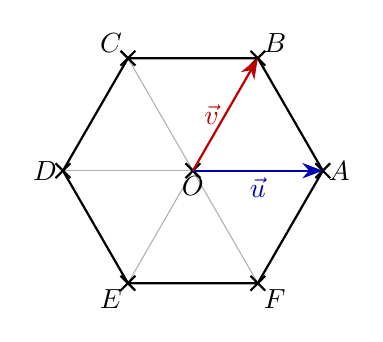
\begin{tikzpicture}[x=0.75cm,y=0.75cm]
\draw[thick] (2.200,0.000) -- (1.100,1.905) -- (-1.100,1.905) -- (-2.200,0.000) -- (-1.100,-1.905) -- (1.100,-1.905) -- cycle;
\draw[gray!60,thin] (0,0) -- (2.200,0.000);
\pt{2.200}{0.000}{A}{west}
\draw[gray!60,thin] (0,0) -- (1.100,1.905);
\pt{1.100}{1.905}{B}{south west}
\draw[gray!60,thin] (0,0) -- (-1.100,1.905);
\pt{-1.100}{1.905}{C}{south east}
\draw[gray!60,thin] (0,0) -- (-2.200,0.000);
\pt{-2.200}{0.000}{D}{east}
\draw[gray!60,thin] (0,0) -- (-1.100,-1.905);
\pt{-1.100}{-1.905}{E}{north east}
\draw[gray!60,thin] (0,0) -- (1.100,-1.905);
\pt{1.100}{-1.905}{F}{north west}
\pt{0}{0}{O}{north}
\draw[vecu] (0,0) -- (2.2,0.0) node[midway,below=1pt,inner sep=1pt] {$\vec u$};
\draw[vecv] (0,0) -- (1.1000000000000003,1.905255888325765) node[midway,left=1pt,inner sep=1pt] {$\vec v$};

\end{tikzpicture}
\end{document}
